\section{Antecedentes}



\begin{frame}{Antecedentes, estimación de RUL}
    \begin{block}{RUL $\Rightarrow$ Serie de tiempo}
    \begin{figure}[!h]
        \centering
		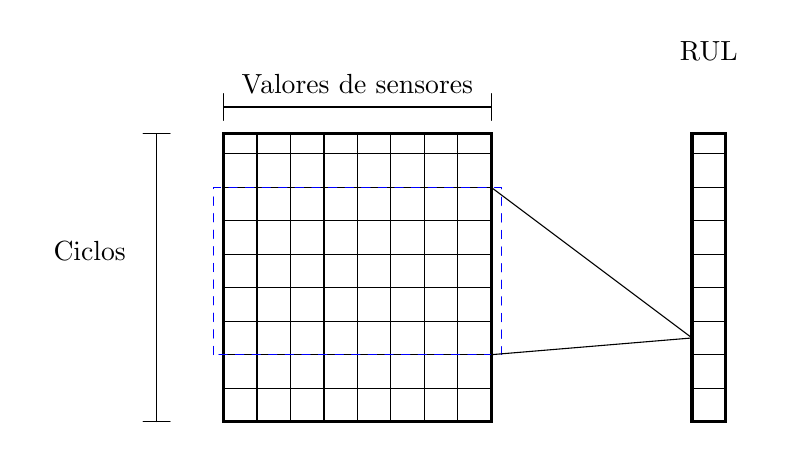
\begin{tikzpicture}[scale=.85,cap=round] 
        %\includegraphics[scale=0.2]{imagenes/cuca_bn.jpg}
		%\node at (-2.5.5,5.5){\begin{tabular}{c}input image\\or input feature map\end{tabular}};
		
		\begin{scope}[
    	yshift=0,every node/.append style={
    	    yslant=0,xslant=0},yslant=0,xslant=0
    	             ]
        \fill[white,fill opacity=.9] (-4,0) rectangle (0,4.3);
        \draw[black,very thick] (-4,0) rectangle (0,4.3);
        \draw[step=5mm, black] (-4,0) grid (0,4.3);
        \end{scope}
        
        \begin{scope}[
    	yshift=0,every node/.append style={
    	    yslant=0,xslant=0},yslant=0,xslant=0
    	             ]
    	%\fill[white,fill opacity=.9] (0,0) rectangle (5,5);
    	%\draw[step=10mm, black] (1,1) grid (4,4);
    	%\draw[black,very thick] (1,1) rectangle (4,4);
    	%\draw[blue,dashed] (-4.15,-0.15) rectangle (0.15,1);
    	\draw[blue,dashed] (-4.15,1) rectangle (0.15,3.5);

        \end{scope}

		
		\draw (0,3.5) -- (3,1.25);%proyeccion 1
		\draw (0,1) -- (3,1.25);%proyeccion 1
		
		\begin{scope}[
    	yshift=0,every node/.append style={
    	    yslant=0,xslant=0},yslant=0,xslant=0
    	             ]
        \fill[white,fill opacity=.9] (3,0) rectangle (3.5,4.3);
        \draw[black,very thick] (3,0) rectangle (3.5,4.3);
        \draw[step=5mm, black] (3,0) grid (3.5,4.3);
        \end{scope}

		\node at (-6,2.5){\begin{tabular}{c}Ciclos\end{tabular}};
		\draw (-5,0) -- (-5,4.3);%
		\draw (-4.8,0) -- (-5.2,0);%
		\draw (-4.8,4.3) -- (-5.2,4.3);%
		
		\node at (-2,5){\begin{tabular}{c}Valores de sensores\end{tabular}};
		\draw (-4,4.7) -- (0,4.7);%
		\draw (-4,4.5) -- (-4,4.9);%
		\draw (0,4.5) -- (0,4.9);%
		
		
		%\node at (-2,5.5){\begin{tabular}{c}\textbf{Matriz de entrada}\end{tabular}};
		\node at (3.25,5.5){\begin{tabular}{c}RUL\end{tabular}};
        
	\end{tikzpicture}
		\caption{Relación entre una serie de tiempo y la RUL dentro del total de datos en la vida de una máquina. La linea punteda indica la serie de tiempo a la cual se le asocia una RUL.}
		\label{CNN}
\end{figure}
    \end{block}
\end{frame}



%perceptrón 
\begin{frame}{Antecedentes, estimación de RUL}
    \begin{block}{Una red neuronal puede relacionar ambas cosas,}
    \begin{figure}[htbp]
\centering
\begin{tikzpicture}[scale=.7,cap=round]
% Styles
\tikzstyle{information text}=[text badly centered] 
% The graphic
\begin{scope}
\pgfsetarrowsend{stealth'}
\pgfsetlinewidth{1pt}

%comentarios
%\draw (7.5,-1.4) -- (7.5,-.25)
%node[below=.9cm,text width=3cm,style=information text]
%{\small $w_{0}$ };


\node at (-3.5,3){\begin{tabular}{c}Entrada\end{tabular}};
\node at (-3.5,2.2){\begin{tabular}{c}de datos\end{tabular}};


\draw (5.5,3) -- (7.7,3)
node[below=.9cm,text width=3cm, style=information text]
{};
\draw (9.3,3) -- (11,3)
node[below=.9cm,text width=3cm, style=information text]
{};
\end{scope}

% draw the nodes

\foreach \x in {-2}
\foreach \y in {-1,0,1,2,3,4,5,6,7} {
\draw (\x,\y) circle (0.1cm);
}

\foreach \x in {4.7}
\foreach \y in {3} {
\draw (\x,\y) circle (0.7cm);
}

\foreach \x in {8.5}
\foreach \y in {3} {
\draw (\x,\y) circle (0.7cm);
}

\draw (4.7,4.7) -- (4.7,4.7)
node[below=.9cm,text width=3cm,style=information text]
{\semihuge $\sum$ };

\draw (8.5,4.7) -- (8.5,4.7)
node[below=.9cm,text width=3cm,style=information text]
{\huge $\sigma$ };

\draw (10.5,3.7)
node[below=.9cm,text width=3cm,style=information text]
{\small Estimación };

% we add the lines for the nodes starting in y 2,3, and 4

\foreach \xa / \xb in {4.4 / -1.9}
\foreach \ya / \yb in {3/-1,3/0,3/1,3/2,3/4,3/5,3/6,3/7} {
\draw (\xa,\ya) -- (\xb,\ya);
\draw (\xa,\ya) -- (\xb,\yb);
}



\end{tikzpicture}
\caption[]%
{Flujo de información y estructura típica de un Perceptrón. \cite{NN}.}
\label{F:Perceptron}
\end{figure}

\end{block}
\end{frame}

\begin{frame}{Antecedentes, redes neuronales}
\begin{figure}
	\centering
	\subfigure{
    		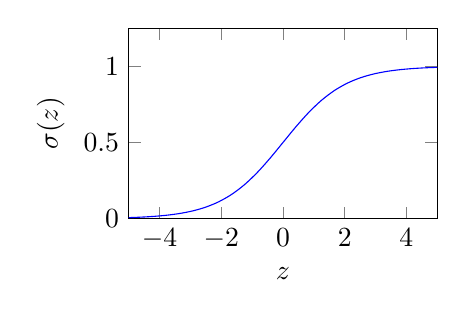
\begin{tikzpicture}
			\begin{axis}[width=5.5cm,height=4cm,ylabel=$\sigma(z)$,xlabel=$z$,ymin=0,ymax=1.25,xmin=-5,xmax=5]
				\addplot[blue,smooth] {1/(1+exp(-x))};
			\end{axis}
		\end{tikzpicture}
	}

	\subfigure{
		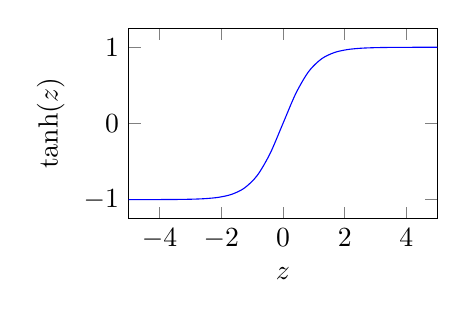
\begin{tikzpicture}
			\begin{axis}[width=5.5cm,height=4cm,ylabel=$\tanh(z)$,xlabel=$z$,ymin=-1.25,ymax=1.25,xmin=-5,xmax=5]
				\addplot[blue,smooth] {tanh(x)};
			\end{axis}
		\end{tikzpicture}
	}

    	
\end{figure}
\end{frame}


%MLP 1
\begin{frame}{Antecedentes, redes neuronales}

\begin{block}{Podemos unir muchos perceptrones,}

\begin{figure}

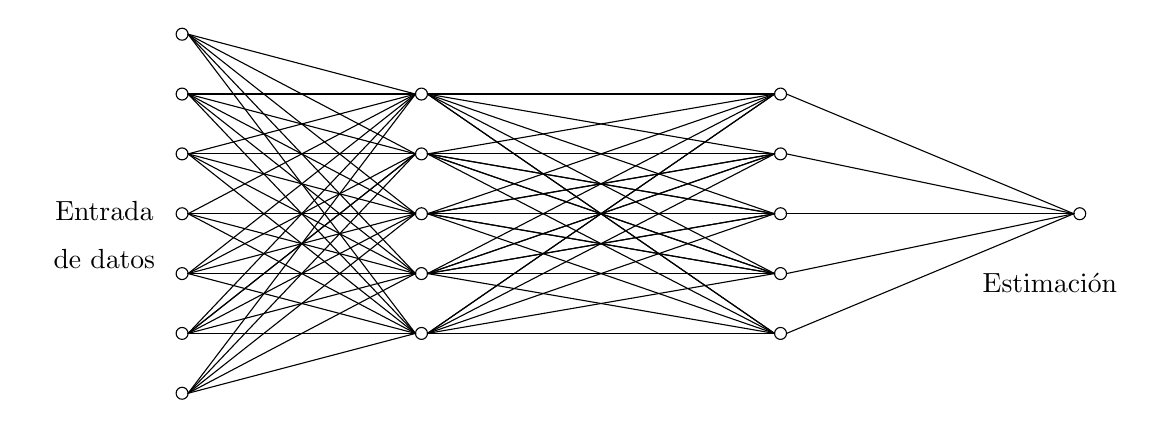
\begin{tikzpicture}[scale=.76,cap=round]
% Styles
\tikzstyle{information text}=[text badly centered] 

% draw the nodes

\foreach \x in {1}
\foreach \y in {0,1,2,3,4,5,6} {
\draw (\x,\y) circle (0.1cm);
}
\foreach \x in {16}
\foreach \y in {3} {
\draw (\x,\y) circle (0.1cm);
}
\foreach \x in {5,11}
\foreach \y in {1,2,3,4,5} {
\draw (\x,\y) circle (0.1cm);
}
% we add the lines for the nodes starting in y 2,3, and 4
\foreach \xa / \xb in {5.1 / 10.9 , 10.9 / 5.1}
\foreach \ya / \yb / \yc / \yd / \ye in {2 / 3 / 4 / 5 / 1, 3 / 4 / 5 / 1 /
2, 4 / 5 / 1 / 2 / 3} {
\draw (\xa,\ya) -- (\xb,\ya);
\draw (\xa,\ya) -- (\xb,\yb);
\draw (\xa,\ya) -- (\xb,\yc);
\draw (\xa,\ya) -- (\xb,\yd);
\draw (\xa,\ya) -- (\xb,\ye);
}
% add remaining lines from y1 to y5
\foreach \xa / \xb in {5.1 / 10.9 , 10.9 / 5.1}
\foreach \ya / \yb in {1 / 5, 5 / 1} {
\draw (\xa,\ya) -- (\xb,\ya);
\draw (\xa,\ya) -- (\xb,\yb);
}

% add remaining lines from y1 to y5
\foreach \xa / \xb in { 4.9/1.1}
\foreach \ya / \yb in {1/0,1/2,1/3,1/4,1/5,1/6,2/0,2/1,2/3,2/4,2/5,2/6,3/0,3/1,3/2,3/4,3/5,3/6,
4/0,4/1,4/2,4/,4/5,4/6,5/0,5/1,5/2,5/3,5/4,5/6} {
\draw (\xa,\ya) -- (\xb,\ya);
\draw (\xa,\ya) -- (\xb,\yb);
}

% add remaining lines from y1 to y5
\foreach \xa / \xb in { 15.9 / 11.1}
\foreach \ya / \yb in {3/1,3/2,3/3,3/4,3/5} {
\draw (\xa,\ya) -- (\xb,\ya);
\draw (\xa,\ya) -- (\xb,\yb);
}

\node at (-0.3,3){\begin{tabular}{c}Entrada\end{tabular}};
\node at (-0.3,2.2){\begin{tabular}{c}de datos\end{tabular}};
\node at (15.5,1.8){\begin{tabular}{c}Estimación\end{tabular}};


\end{tikzpicture}
\caption{Perceptrón de múltiples capas para regresión logística.}
\label{fig:MLP}

\end{figure}
\end{block}

\end{frame}




%MLP 0
\begin{frame}{Antecedentes, redes neuronales}

\begin{figure}

\begin{tikzpicture}[scale=.8,cap=round]
% Styles
\tikzstyle{information text}=[text badly centered] 

% draw the nodes

\foreach \x in {1}
\foreach \y in {0,1,2,3,4,5,6} {
\draw (\x,\y) circle (0.1cm);
}
\foreach \x in {16}
\foreach \y in {3} {
\draw (\x,\y) circle (0.1cm);
}
\foreach \x in {5,11}
\foreach \y in {1,2,3,4,5} {
\draw (\x,\y) circle (0.1cm);
}
%fill neuron
\draw (5,2) circle (0.1cm);
\foreach \x in {11}
\foreach \y in {1,2,3,4,5} {
\draw (\x,\y) circle (0.1cm);
}




\node at (-0.3,3){\begin{tabular}{c}Entrada\end{tabular}};
\node at (-0.3,2.2){\begin{tabular}{c}de datos\end{tabular}};
\node at (15.5,1.8){\begin{tabular}{c}Estimación\end{tabular}};



\end{tikzpicture}


\end{figure}

\end{frame}


%MLP 1
\begin{frame}{Antecedentes, redes neuronales}

\begin{figure}

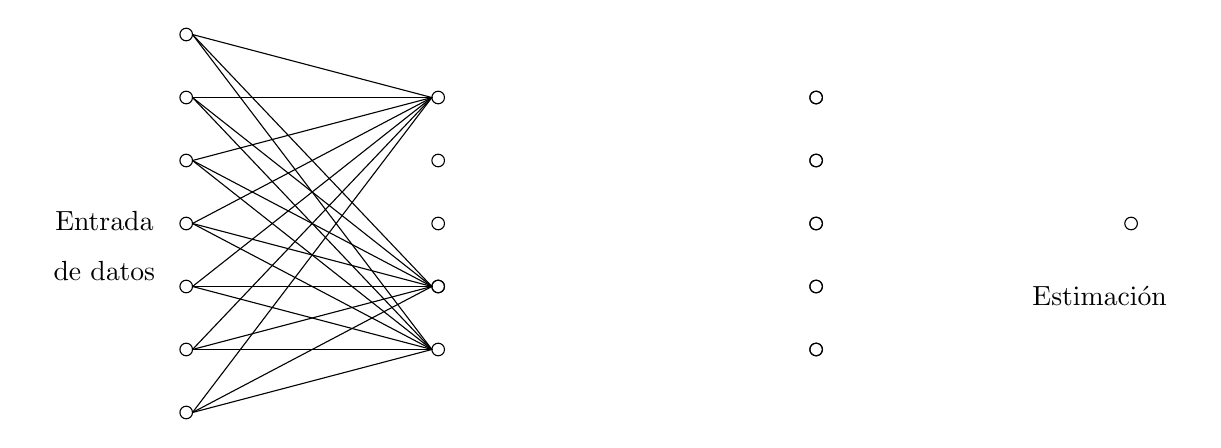
\begin{tikzpicture}[scale=.8,cap=round]
% Styles
\tikzstyle{information text}=[text badly centered] 

% draw the nodes

\foreach \x in {1}
\foreach \y in {0,1,2,3,4,5,6} {
\draw (\x,\y) circle (0.1cm);
}
\foreach \x in {16}
\foreach \y in {3} {
\draw (\x,\y) circle (0.1cm);
}
\foreach \x in {5,11}
\foreach \y in {1,2,3,4,5} {
\draw (\x,\y) circle (0.1cm);
}
%fill neuron
\draw (5,2) circle (0.1cm);
\foreach \x in {11}
\foreach \y in {1,2,3,4,5} {
\draw (\x,\y) circle (0.1cm);
}


%fill path
%primera capa
\foreach \y in {0,1,2,3,4,5,6} {
\draw(1.1,\y) -- (4.9,2);
}
\foreach \y in {0,1,2,3,4,5,6} {
\draw(1.1,\y) -- (4.9,1);
}
\foreach \y in {0,1,2,3,4,5,6} {
\draw(1.1,\y) -- (4.9,5);
}


\node at (-0.3,3){\begin{tabular}{c}Entrada\end{tabular}};
\node at (-0.3,2.2){\begin{tabular}{c}de datos\end{tabular}};
\node at (15.5,1.8){\begin{tabular}{c}Estimación\end{tabular}};



\end{tikzpicture}


\end{figure}

\end{frame}

%MLP 2
\begin{frame}{Antecedentes, redes neuronales}

\begin{figure}

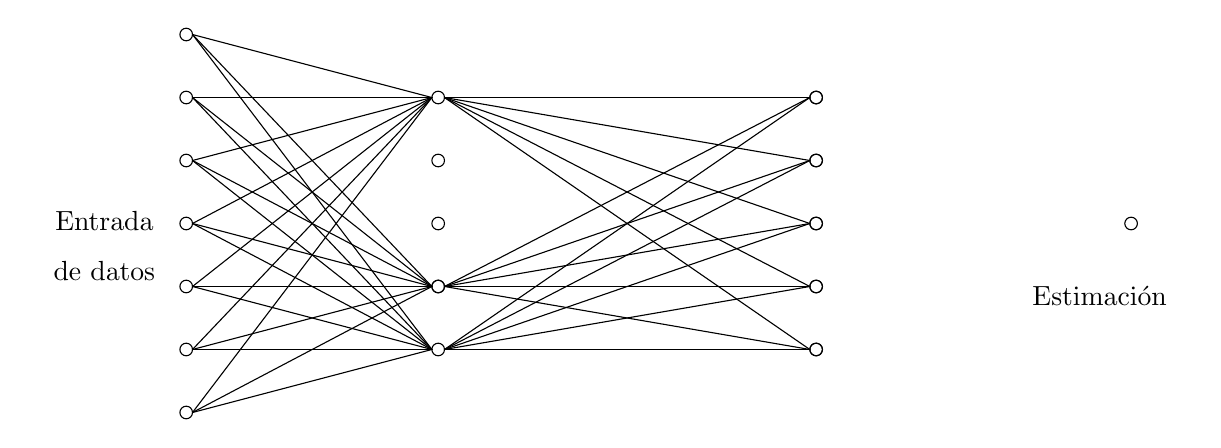
\begin{tikzpicture}[scale=.8,cap=round]
% Styles
\tikzstyle{information text}=[text badly centered] 

% draw the nodes

\foreach \x in {1}
\foreach \y in {0,1,2,3,4,5,6} {
\draw (\x,\y) circle (0.1cm);
}
\foreach \x in {16}
\foreach \y in {3} {
\draw (\x,\y) circle (0.1cm);
}
\foreach \x in {5,11}
\foreach \y in {1,2,3,4,5} {
\draw (\x,\y) circle (0.1cm);
}
%fill neuron
\draw (5,2) circle (0.1cm);
\foreach \x in {11}
\foreach \y in {1,2,3,4,5} {
\draw (\x,\y) circle (0.1cm);
}


%fill path
%primera capa
\foreach \y in {0,1,2,3,4,5,6} {
\draw(1.1,\y) -- (4.9,2);
}
\foreach \y in {0,1,2,3,4,5,6} {
\draw(1.1,\y) -- (4.9,1);
}
\foreach \y in {0,1,2,3,4,5,6} {
\draw(1.1,\y) -- (4.9,5);
}

%segunda capa
\foreach \y in {1,2,3,4,5} {
\draw(5.1,1) -- (10.9,\y);
}
\foreach \y in {1,2,3,4,5} {
\draw(5.1,2) -- (10.9,\y);
}
\foreach \y in {1,2,3,4,5} {
\draw(5.1,5) -- (10.9,\y);
}


\node at (-0.3,3){\begin{tabular}{c}Entrada\end{tabular}};
\node at (-0.3,2.2){\begin{tabular}{c}de datos\end{tabular}};
\node at (15.5,1.8){\begin{tabular}{c}Estimación\end{tabular}};



\end{tikzpicture}


\end{figure}

\end{frame}


%MLP 3
\begin{frame}{Antecedentes, redes neuronales}

\begin{figure}

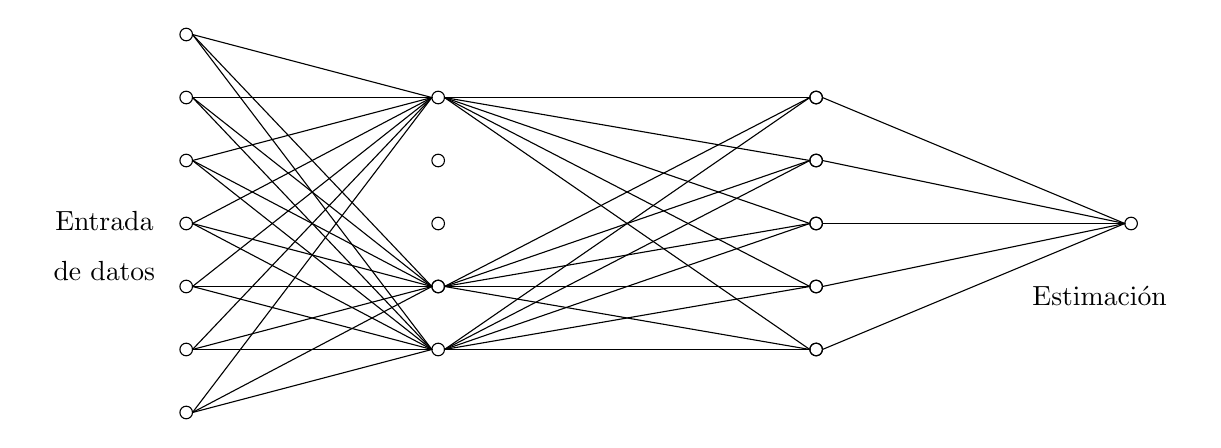
\begin{tikzpicture}[scale=.8,cap=round]
% Styles
\tikzstyle{information text}=[text badly centered] 

% draw the nodes

\foreach \x in {1}
\foreach \y in {0,1,2,3,4,5,6} {
\draw (\x,\y) circle (0.1cm);
}
\foreach \x in {16}
\foreach \y in {3} {
\draw (\x,\y) circle (0.1cm);
}
\foreach \x in {5,11}
\foreach \y in {1,2,3,4,5} {
\draw (\x,\y) circle (0.1cm);
}
%fill neuron
\draw (5,2) circle (0.1cm);
\foreach \x in {11}
\foreach \y in {1,2,3,4,5} {
\draw (\x,\y) circle (0.1cm);
}


%fill path
%primera capa
\foreach \y in {0,1,2,3,4,5,6} {
\draw(1.1,\y) -- (4.9,2);
}
\foreach \y in {0,1,2,3,4,5,6} {
\draw(1.1,\y) -- (4.9,1);
}
\foreach \y in {0,1,2,3,4,5,6} {
\draw(1.1,\y) -- (4.9,5);
}

%segunda capa
\foreach \y in {1,2,3,4,5} {
\draw(5.1,1) -- (10.9,\y);
}
\foreach \y in {1,2,3,4,5} {
\draw(5.1,2) -- (10.9,\y);
}
\foreach \y in {1,2,3,4,5} {
\draw(5.1,5) -- (10.9,\y);
}

% tercera capa
\foreach \xa / \xb in { 15.9 / 11.1}
\foreach \ya / \yb in {3/1,3/2,3/3,3/4,3/5} {

\draw (\xa,\ya) -- (\xb,\yb);
}

\node at (-0.3,3){\begin{tabular}{c}Entrada\end{tabular}};
\node at (-0.3,2.2){\begin{tabular}{c}de datos\end{tabular}};
\node at (15.5,1.8){\begin{tabular}{c}Estimación\end{tabular}};



\end{tikzpicture}


\end{figure}

\end{frame}
%%%%%%%%%%%%%%
%%%%%%%%%%%%%%
%%%%%%%%%%%%%%


\begin{frame}{Antecedentes, redes neuronales}
    \begin{block}{Retropropagación \cite{BPTT},}
    \begin{figure}
        \centering
        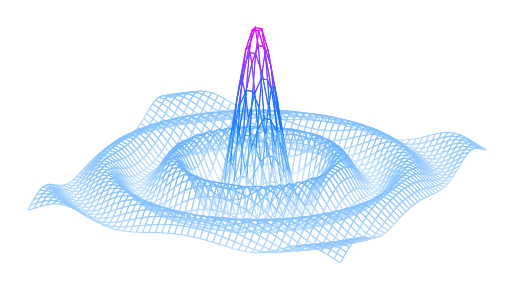
\begin{tikzpicture}[scale=0.85]
        
\begin{axis}[
    hide axis,
    colormap/cool,
]
\addplot3[
    mesh,
    samples=50,
    domain=-8:8,
]
{ cos(deg(sqrt(x^2+y^2)))*sin(deg(sqrt(x^2+y^2)))/sqrt(x^2+y^2)};
\end{axis}
\end{tikzpicture}
        \caption{Superficie creada por distintas posibilidades de pesos y un error determinado.}
        \label{fig:surface}
    \end{figure}
    \end{block}
    
    \begin{block}{Los optimizadores ajustan los pesos}
    \begin{itemize}
    \item Cuanto se ajusta, $\bigtriangleup w_{ij} = -\eta \frac{\partial E_{n}}{\partial w_{ij}}$.
    \item Cómo se ajusta, $w_{ij} = w_{ij} + \bigtriangleup w_{ij}$.
    \end{itemize}
    \end{block}
\end{frame}



\begin{frame}{Antecedentes, redes neuronales}
    \begin{block}{Redes Neuronales Convolucionales \cite{CNN},}
    \begin{figure}
        
        \centering
		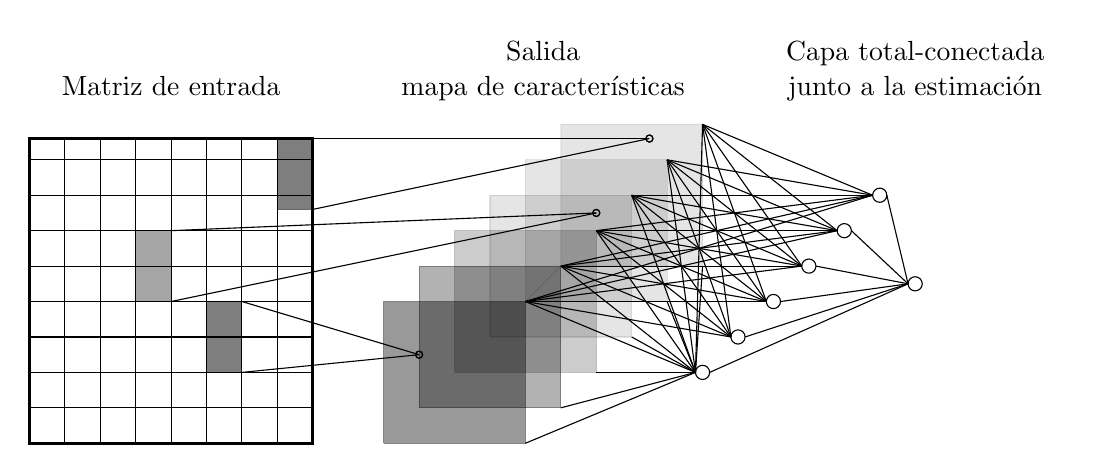
\begin{tikzpicture}[scale=0.9]
		
		\begin{scope}[
    	yshift=0,every node/.append style={
    	    yslant=0,xslant=0},yslant=0,xslant=0
    	             ]
        \fill[white,fill opacity=.9] (-4,0) rectangle (0,4.3);
        \draw[black,very thick] (-4,0) rectangle (0,4.3);
        \draw[step=5mm, black] (-4,0) grid (0,4.3);
        \end{scope}
        
        \begin{scope}[
    	yshift=0,every node/.append style={
    	    yslant=0,xslant=0},yslant=0,xslant=0
    	             ]
    	%\fill[white,fill opacity=.9] (0,0) rectangle (5,5);
    	%\draw[step=10mm, black] (1,1) grid (4,4);
    	%\draw[black,very thick] (1,1) rectangle (4,4);
    	%\draw[blue,dashed] (-4.15,-0.15) rectangle (0.15,1);
    	%\draw[blue,dashed] (-4.15,3.5) rectangle (0.15,4.5);

        \end{scope}
    	
        	
	
		%\draw (-3,1) -- (0,1) -- (0,4.3) -- (-3,4.3) -- (-3,1);%imagen
		
	    \draw [fill=black,opacity=0.5,draw=black](0,3.3) -- (-0.5,3.3) -- (-0.5,4.3) -- (0,4.3) -- (0,3.3);%kernel 1
		\draw [fill=black,opacity=0.35,draw=black](-2,3) -- (-2.5,3) -- (-2.5,2) -- (-2,2) -- (-2,3);%kernel 3
		\draw [fill=black,opacity=0.5,draw=black](-1,1) -- (-1.5,1) -- (-1.5,2) -- (-1,2) -- (-1,1);%kernel 2
		
		\draw (-2.,3) -- (4,3.25);%proyeccion 1
		\draw (-2.,2.0) -- (4,3.25);%proyeccion 1

		\draw (0,4.3) -- (4.75,4.3);%proyeccion 3
		\draw (0,3.3) -- (4.75,4.3);%proyeccion 3
		
		\draw (-1.,2) -- (1.5,1.25);%proyeccion 2
		\draw (-1.,1.0) -- (1.5,1.25);%proyeccion 2
		
		\node at (-2,5){\begin{tabular}{c}Matriz de entrada\end{tabular}};
		\node at (3.25,5.5){\begin{tabular}{c}Salida\end{tabular}};
		\node at (3.25,5){\begin{tabular}{c}mapa de características\end{tabular}};
		\node at (8.5,5.5){\begin{tabular}{c}Capa total-conectada\end{tabular}};
		\node at (8.5,5){\begin{tabular}{c}junto a la estimación\end{tabular}};
		
		
		
		\draw[fill=black,opacity=0.1,draw=black] (3.5,2.5) -- (5.5,2.5) -- (5.5,4.5) -- (3.5,4.5) -- (3.5,2.5)--(3,2);
		\draw[fill=black,opacity=0.1,draw=black] (3,2) -- (5,2) -- (5,4) -- (3,4) -- (3,2);
		\draw[fill=black,opacity=0.1,draw=black] (2.5,1.5) -- (4.5,1.5) -- (4.5,3.5) -- (2.5,3.5) -- (2.5,1.5);
		\draw[fill=black,opacity=0.2,draw=black] (2,1) -- (4,1) -- (4,3) -- (2,3) -- (2,1);
		\draw[fill=black,opacity=0.3,draw=black] (1.5,0.5) -- (3.5,0.5) -- (3.5,2.5) -- (1.5,2.5) -- (1.5,0.5);
		\draw[fill=black,opacity=0.4,draw=black] (1,0) -- (3,0) -- (3,2) -- (1,2) -- (1,0);
		
		
        \draw (4.75,4.3) circle (0.05cm);
        \draw (4,3.25) circle (0.05cm);
        \draw (1.5,1.25) circle (0.05cm);
        
        %full-connected layer
        \draw (4.75,4.3) circle (0.05cm);
        \draw (4,3.25) circle (0.05cm);
        \draw (1.5,1.25) circle (0.05cm);
        
        \draw (8.5,2.25) circle (0.1cm);
        
        \draw (8,3.5) circle (0.1cm);
        \draw (7.5,3) circle (0.1cm);
        \draw (7,2.5) circle (0.1cm);
        \draw (6.5,2) circle (0.1cm);
        \draw (6,1.5) circle (0.1cm);
        \draw (5.5,1) circle (0.1cm);
        
        %conections in first nodo
        \draw (5.5,4.5) -- (7.9,3.5);
        \draw (5,4) -- (7.9,3.5);
        \draw (4.5,3.5) -- (7.9,3.5);
        \draw (4,3) -- (7.9,3.5);
        \draw (3.5,2.5) -- (7.9,3.5);
        \draw (3,2) -- (7.9,3.5);
        
        
        
        %conections in second nodo
        \draw (5.5,4.5) -- (7.4,3);
        \draw (5,4) -- (7.4,3);
        \draw (4.5,3.5) -- (7.4,3);
        \draw (4,3) -- (7.4,3);
        \draw (3.5,2.5) -- (7.4,3);
        \draw (3,2) -- (7.4,3);
        
        %conections in third nodo
        \draw (5.5,4.5) -- (6.9,2.5);
        \draw (5,4) -- (6.9,2.5);
        \draw (4.5,3.5) -- (6.9,2.5);
        \draw (4,3) -- (6.9,2.5);
        \draw (3.5,2.5) -- (6.9,2.5);
        \draw (3,2) -- (6.9,2.5);
        
        %conections in fourth nodo
        \draw (5.5,4.5) -- (6.4,2);
        \draw (5,4) -- (6.4,2);
        \draw (4.5,3.5) -- (6.4,2);
        \draw (4,3) -- (6.4,2);
        \draw (3.5,2.5) -- (6.4,2);
        \draw (3,2) -- (6.4,2);
        
        %conections in fifth nodo
        \draw (5.5,4.5) -- (5.9,1.5);
        \draw (5,4) -- (5.9,1.5);
        \draw (4.5,3.5) -- (5.9,1.5);
        \draw (4,3) -- (5.9,1.5);
        \draw (3.5,2.5) -- (5.9,1.5);
        \draw (3,2) -- (5.9,1.5);
        
        
        %conections in sixth nodo
        \draw (5.5,4.5) -- (5.4,1);
        \draw (5,4) -- (5.4,1);
        \draw (4.5,3.5) -- (5.4,1);
        \draw (4,3) -- (5.4,1);
        \draw (3.5,2.5) -- (5.4,1);
        \draw (3,2) -- (5.4,1);
        
        \draw (5.5,2.5) -- (5.4,1);
        \draw (5,2) -- (5.4,1);
        \draw (4.5,1.5) -- (5.4,1);
        \draw (4,1) -- (5.4,1);
        \draw (3.5,0.5) -- (5.4,1);
        \draw (3,0) -- (5.4,1);
        
        %conections in last nodo
        \draw (5.6,1) -- (8.4,2.25);
        \draw (6.1,1.5) -- (8.4,2.25);
        \draw (6.6,2) -- (8.4,2.25);
        \draw (7.1,2.5) -- (8.4,2.25);
        \draw (7.6,3) -- (8.4,2.25);
        \draw (8.1,3.5) -- (8.4,2.25);
        
        
	\end{tikzpicture}
	\caption{Modelo estándar de aplicación de redes neuronales convolucionales.}
        \label{fig:CNN}
    \end{figure}
    
    \end{block}
\end{frame}


\begin{frame}{Antecedentes, redes neuronales}
    \begin{block}{Redes neuronales recurrentes (\cite{RNN1} y \cite{RNN2}),}
    \begin{figure}[!h]

   \begin{tikzpicture}[scale=.5]
   \begin{scope}
   \pgfsetarrowsend{stealth'}
   \pgfsetlinewidth{0.1pt}
   %first RNN
   \draw (2,-1.4) -- (2,0.2);
   \draw (2,1.7) -- (2,3.3);
   \draw (2,1.7) .. controls +(2,1.25) and +(2,-0.8)..  (2.1,0.2);
   
   %unroled 1
   \draw (6,-1.4) -- (6,0.2);
   \draw (6,1.7) -- (6,3.3);
   \draw (6.75,1) -- (9.25,1);
   
   %unroled 2
   \draw (10,-1.4) -- (10,0.2);
   \draw (10,1.7) -- (10,3.3);
   \draw (10.75,1) -- (13.25,1);
   
   %unroled 
   \draw (14,-1.4) -- (14,0.2);
   \draw (14,1.7) -- (14,3.3);
   \draw (14.75,1) -- (15.15,1);
\end{scope}
    ;
	%first RNN
	\draw[fill=black,opacity=0.4,draw=black] (2,1) circle (0.7cm);
	\draw (4.4,3.25) -- (4.4,3.25)%(x+2.4,y+1.05)
	node[below=.9cm,text width=3cm,style=information text]
	{\scriptsize RNN };
	\draw (4.7,0.2) -- (4.7,0.2)%cambiar 2.7 (2.7+x,y+1.2)
	node[below=.9cm,text width=3cm,style=information text]
	{\small $x^{(t)}$ };
	\draw (4.7,6.5) -- (4.7,6.8)%cambiar 2.7 (2.7+x,y+1.5)
	node[below=.9cm,text width=3cm,style=information text]
	{\small $y^{(t)}$ };
	\draw (5.5,5) -- (5.5,5)
	node[below=.9cm,text width=3cm,style=information text]
	{\small $h^{(t)}$ };
	\draw (5.5,1.9) -- (5.5,1.9)
	node[below=.9cm,text width=3cm,style=information text]
	{\small $h^{(t-1)}$ };
	\draw (4.7,-1) -- (4.7,-1)%(x+2.7,y)
	node[below=.9cm,text width=3cm,style=information text]
	{\small $(a)$ };
	\draw (2,3.5) circle (0.1cm);
	\draw (2,-1.5) circle (0.1cm);
	\draw[fill=white,opacity=1,draw=black] (3.55, 1) circle (0.1cm);
	
	%unroled 1
	\draw[fill=black,opacity=0.3,draw=black] (6,1) circle (0.7cm);
	\draw (8.4,3.25) -- (8.4,3.25)
	node[below=.9cm,text width=3cm,style=information text]
	{\scriptsize RNN };
	\draw (10.5, 2.8) -- (10.5, 2.8)
	node[below=.9cm,text width=3cm,style=information text]
	{\small $h^{(1)}$ };
	\draw (8.7,0.2) -- (8.7,0.2)
	node[below=.9cm,text width=3cm,style=information text]
	{\small $x^{(1)}$ };
	\draw (8.7,6.8) -- (8.7,6.8)
	node[below=.9cm,text width=3cm,style=information text]
	{\small $y^{(1)}$ };
	\draw (6,3.5) circle (0.1cm);
	\draw (6,-1.5) circle (0.1cm);
	\draw[fill=white,opacity=1,draw=black] (8, 1) circle (0.1cm);
	
	
	%unroled 2
	\draw[fill=black,opacity=0.2,draw=black] (10,1) circle (0.7cm);
	\draw (12.4,3.25) -- (12.4,3.25)
	node[below=.9cm,text width=3cm,style=information text]
	{\scriptsize RNN };
	\draw (14.5, 2.8) -- (14.5, 2.8)
	node[below=.9cm,text width=3cm,style=information text]
	{\small $h^{(2)}$ };
	\draw (12.7,0.2) -- (12.7,0.2)
	node[below=.9cm,text width=3cm,style=information text]
	{\small $x^{(2)}$ };
	\draw (12.7,6.8) -- (12.7,6.8)
	node[below=.9cm,text width=3cm,style=information text]
	{\small $y^{(2)}$ };
	\draw (12.7,-1) -- (12.7,-1)
	node[below=.9cm,text width=3cm,style=information text]
	{\small $(b)$ };
	\draw (10,3.5) circle (0.1cm);
	\draw (10,-1.5) circle (0.1cm);
	\draw[fill=white,opacity=1,draw=black] (12, 1) circle (0.1cm);
	
	%unroled 3
	\draw[fill=black,opacity=0.1,draw=black] (14,1) circle (0.7cm);
	\draw (16.4,3.25) -- (16.4,3.25)
	node[below=.9cm,text width=3cm,style=information text]
	{\scriptsize RNN };
	\draw (17.8, 2.8) -- (17.8, 2.8)
	node[below=.9cm,text width=3cm,style=information text]
	{\small $h^{(3)}$ };
	\draw (16.7,0.2) -- (16.7,0.2)
	node[below=.9cm,text width=3cm,style=information text]
	{\small $x^{(3)}$ };
	\draw (16.7,6.8) -- (16.7,6.8)
	node[below=.9cm,text width=3cm,style=information text]
	{\small $y^{(3)}$ };
	\draw (14,3.5) circle (0.1cm);
	\draw (14,-1.5) circle (0.1cm);
	\draw[fill=white,opacity=1,draw=black] (15.3, 1) circle (0.1cm);
	

	
\end{tikzpicture}
    \caption{Célula de red recurrente. Grafo cíclico tipico $(a)$ que puede ser desplagado en $(b)$ como grafo acíclico. }
    \label{fig:RNN}
\end{figure}

    \end{block}
\end{frame}
%%%%%%%%%%%%%%
%%%%%%%%%%%%%%
%%%%%%%%%%%%%%


\begin{frame}{Antecedentes, redes neuronales}
    \begin{block}{Redes neuronales recurrentes, LSTM \cite{LSTM},}
    \begin{figure}
    \centering
   \begin{tikzpicture}[scale=.6]
   \begin{scope}
   \pgfsetarrowsend{stealth'}
   \pgfsetlinewidth{0.1pt}
   
   
   %unroled 1
   \draw (6,-1.4) -- (6,0.2);
   \draw (6,1.7) -- (6,3.3);
   
   
   %unroled 2
   \draw (10,-1.4) -- (10,0.2);
   \draw (10,1.7) -- (10,3.3);
   %\draw (10.75,1) -- (13.25,1);
   
   %unroled 
   \draw (14,-1.4) -- (14,0.2);
   \draw (14,1.7) -- (14,3.3);
   %\draw (14.75,1) -- (15.15,1);
\end{scope}
    ;
	
	
	%unroled 1
	\draw[fill=black,opacity=0.3,draw=black] (6,1) circle (0.7cm);
	\draw (7.85,2.9) -- (7.85,2.9)
	node[below=.9cm,text width=3cm,style=information text]
	{\scriptsize LSTM };
	
	
	\draw (8.2,-0.2) -- (8.2,-0.2)
	node[below=.9cm,text width=3cm,style=information text]
	{\small $x^{(1)}$ };
	\draw (8.2,6.5) -- (8.2,6.5)
	node[below=.9cm,text width=3cm,style=information text]
	{\small $y^{(1)}$ };
	\draw (6,3.5) circle (0.1cm);
	\draw (6,-1.5) circle (0.1cm);
	
	%flecha de transferencia
	
	\begin{scope}
   \pgfsetarrowsend{stealth'}
   \pgfsetlinewidth{0.1pt}
	\draw (6.75,1.3) -- (9.25,1.3);
	\draw (6.75,0.7) -- (9.25,0.7);
	
	\end{scope}
	\draw[fill=white,opacity=1,draw=black] (8, 1.3) circle (0.1cm);%circulo tranferencia
	\draw[fill=white,opacity=1,draw=black] (8, 0.7) circle (0.1cm);%circulo tranferencia
	
	%informacion tranferida
	\draw (10, 2) -- (10, 2)
	node[below=.9cm,text width=3cm,style=information text]
	{\small $h^{(1)}$ };
	\draw (10, 4.1) -- (10, 4.1)
	node[below=.9cm,text width=3cm,style=information text]
	{\small $c^{(1)}$ };
	
	
	%unroled 2
	\draw[fill=black,opacity=0.2,draw=black] (10,1) circle (0.7cm);
	\draw (11.85,2.9) -- (11.85,2.9)
	node[below=.9cm,text width=3cm,style=information text]
	{\scriptsize LSTM };
	
	\draw (12.2,-0.2) -- (12.2,-0.2)
	node[below=.9cm,text width=3cm,style=information text]
	{\small $x^{(2)}$ };
	\draw (12.2,6.5) -- (12.2,6.5)
	node[below=.9cm,text width=3cm,style=information text]
	{\small $y^{(2)}$ };
	
	\draw (10,3.5) circle (0.1cm);
	\draw (10,-1.5) circle (0.1cm);
	%\draw[fill=white,opacity=1,draw=black] (12, 1) circle (0.1cm);
	
	%flecha de transferencia
	
	\begin{scope}
   \pgfsetarrowsend{stealth'}
   \pgfsetlinewidth{0.1pt}
	\draw (10.75,1.3) -- (13.25,1.3);
	\draw (10.75,0.7) -- (13.25,0.7);
	
	\end{scope}
	\draw[fill=white,opacity=1,draw=black] (12, 1.3) circle (0.1cm);%circulo tranferencia
	\draw[fill=white,opacity=1,draw=black] (12, 0.7) circle (0.1cm);%circulo tranferencia
	
	%informacion tranferida
	\draw (14, 2) -- (14, 2)
	node[below=.9cm,text width=3cm,style=information text]
	{\small $h^{(2)}$ };
	\draw (14, 4.1) -- (14, 4.1)
	node[below=.9cm,text width=3cm,style=information text]
	{\small $c^{(2)}$ };
	
	%unroled 3
	\draw[fill=black,opacity=0.1,draw=black] (14,1) circle (0.7cm);
	\draw (15.85,2.9) -- (15.85,2.9)
	node[below=.9cm,text width=3cm,style=information text]
	{\scriptsize LSTM };
	
	\draw (16.2,-0.2) -- (16.2,-0.2)
	node[below=.9cm,text width=3cm,style=information text]
	{\small $x^{(3)}$ };
	\draw (16.2,6.5) -- (16.2,6.5)
	node[below=.9cm,text width=3cm,style=information text]
	{\small $y^{(3)}$ };
	\draw (14,3.5) circle (0.1cm);
	\draw (14,-1.5) circle (0.1cm);
	
	
	%flecha de transferencia
	
	\begin{scope}
   \pgfsetarrowsend{stealth'}
   \pgfsetlinewidth{0.1pt}
	\draw (14.75,1.3) -- (15.15,1.3);
	\draw (14.75,0.7) -- (15.15,0.7);
	
	\end{scope}
	\draw[fill=white,opacity=1,draw=black] (15.3, 1.3) circle (0.1cm);%circulo tranferencia
	\draw[fill=white,opacity=1,draw=black] (15.3, 0.7) circle (0.1cm);%circulo tranferencia
	
	%informacion tranferida
	\draw (17.8, 2) -- (17.8, 2)
	node[below=.9cm,text width=3cm,style=information text]
	{\small $h^{(3)}$ };
	\draw (17.8, 4.1) -- (17.8, 4.1)
	node[below=.9cm,text width=3cm,style=information text]
	{\small $c^{(3)}$ };
	
	

	
\end{tikzpicture}
    \caption{Flujo de información en célula LSTM. }
    \label{fig:RNN}
\end{figure}

    \end{block}
\end{frame}


\begin{frame}{Antecedentes, redes neuronales}
    \begin{block}{Redes neuronales recurrentes, JANET \cite{janet},}
    \begin{figure}
   \centering
   \begin{tikzpicture}[scale=.6]
   \begin{scope}
   \pgfsetarrowsend{stealth'}
   \pgfsetlinewidth{0.1pt}
   
   
   %unroled 1
   \draw (6,-1.4) -- (6,0.2);
   
   \draw (6.75,1) -- (9.25,1);
   
   %unroled 2
   \draw (10,-1.4) -- (10,0.2);
   
   \draw (10.75,1) -- (13.25,1);
   
   %unroled 
   \draw (14,-1.4) -- (14,0.2);
   
   \draw (14.75,1) -- (15.15,1);
\end{scope}
    ;
	
	
	%unroled 1
	\draw[fill=black,opacity=0.3,draw=black] (6,1) circle (0.7cm);
	\draw (7.9,2.9) -- (7.9,2.9)
	node[below=.9cm,text width=3cm,style=information text]
	{\tiny JANET };
	\draw (10, 2.3) -- (10, 2.3)
	node[below=.9cm,text width=3cm,style=information text]
	{\small $c^{(1)}$ };
	\draw (8.2,-0.2) -- (8.2,-0.2)
	node[below=.9cm,text width=3cm,style=information text]
	{\small $x^{(1)}$ };
	
	
	\draw (6,-1.5) circle (0.1cm);
	\draw[fill=white,opacity=1,draw=black] (8, 1) circle (0.1cm);
	
	
	%unroled 2
	\draw[fill=black,opacity=0.2,draw=black] (10,1) circle (0.7cm);
	\draw (11.9,2.9) -- (11.9,2.9)
	node[below=.9cm,text width=3cm,style=information text]
	{\tiny JANET};
	\draw (14, 2.3) -- (14, 2.3)
	node[below=.9cm,text width=3cm,style=information text]
	{\small $c^{(2)}$ };
	\draw (12.2,-0.2) -- (12.2,-0.2)
	node[below=.9cm,text width=3cm,style=information text]
	{\small $x^{(2)}$ };
	
	
	
	\draw (10,-1.5) circle (0.1cm);
	\draw[fill=white,opacity=1,draw=black] (12, 1) circle (0.1cm);
	
	%unroled 3
	\draw[fill=black,opacity=0.1,draw=black] (14,1) circle (0.7cm);
	\draw (15.9,2.9) -- (15.9,2.9)
	node[below=.9cm,text width=3cm,style=information text]
	{\tiny JANET};
	\draw (17.3, 2.3) -- (17.3, 2.3)
	node[below=.9cm,text width=3cm,style=information text]
	{\small $c^{(3)}$ };
	\draw (16.2,-0.2) -- (16.2,-0.2)
	node[below=.9cm,text width=3cm,style=information text]
	{\small $x^{(3)}$ };
	
	
	\draw (14,-1.5) circle (0.1cm);
	\draw[fill=white,opacity=1,draw=black] (15.3, 1) circle (0.1cm);
	

	
\end{tikzpicture}
    \caption{Flujo de información en JANET. }
    \label{fig:RNN}
\end{figure}

    \end{block}
\end{frame}

\begin{frame}{Antecedentes, redes neuronales recurrentes convolucionales}
    \begin{block}{Aplicable de forma directa similar a una CNN,}
    \begin{figure}
        \centering
        \includegraphics[scale=0.4]{animate/conv_lstm.png}
        \caption{Aplicación directa de una ConvRNN para la predicción.}
        \label{fig:convrnn}
    \end{figure}
    \end{block}
\end{frame}

\begin{frame}{Antecedentes, redes neuronales recurrentes convolucionales}
    \begin{block}{Como Codificadora-Decodificadora (\cite{convlstm}, \cite{E-D1} y \cite{E-D2}),}
    \begin{figure}
        \centering
        \includegraphics[scale=0.4]{animate/Codificador-Decodificador.png}
        \caption{Aplicación de ConvRNN como Codificadora-Decodificadora para la predicción.}
        \label{fig:my_label}
    \end{figure}
    \end{block}
\end{frame}

\begin{frame}{Antecedentes, Base de datos}
\begin{block}{Turbofan}

\begin{figure}[!h]
		\centering
		\includegraphics[scale=0.5]{animate/turbofan31.png}
		\caption{Descripción de partes de un turbofan donde se especifica el ducto de bypass. \cite{bypass_nasa}. }
		\label{logofcfm}
	\end{figure}
\end{block}
\end{frame}
%foto turbofan: https://www.grc.nasa.gov/www/k-12/Missions/Jim/Project2_act.htm


\begin{frame}{Antecedentes, Base de datos}
\begin{block}{C-MAPSS \cite{metricas-rmse}}
\begin {itemize}
    \item Datos como velocidad, presión, temperatura, etc.
    \pause
    \item Ruido blanco.
    \pause
    \item Operación y fallas.
    \pause
    \item Cantidad de datos.
\end {itemize}
\end{block}
\end{frame}

\begin{frame}{Antecedentes, Medición de exactitud}
    \begin{figure}
        \centering
        \includegraphics[scale=0.3]{animate/error_metricas_evaluacion.png}
        \caption{Asignación de puntaje y exactitud de un modelo según su error. \cite{metricas-rmse}.}
        \label{fig:rmse-score}
    \end{figure}
\end{frame}
